\section{REST API}
\label{sec:restapi}
The REST API was built and designed as remote-acting standalone web application, running on Node's servers-side JavaScript engine. Apart from specificly reserved firewall ports, the project is only dependent on a Node.js install, every other dependency may be installed using npm, regardless on the used operating system.

By extending any desired Node.js Dockerfile\footnote{\url{https://hub.docker.com/\_/node/} -- Official repository for Node.js on Docker Hub.}, it may be even run as autonomous Docker container and therefore multiplied for better load balancing based on the current HTTP load extent.


%% Screenshot of console log output after running artillery
\begin{figure}[h] % h-ere, t-op, b-ottom, p-age
    \centering
    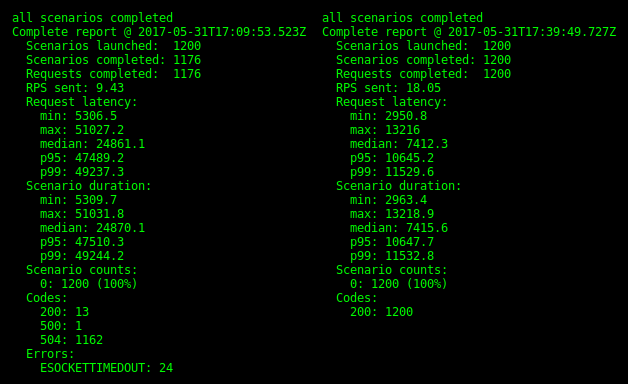
\includegraphics[width=0.9\textwidth]{pen_test.png}
    \caption{Screenshots of two command line outputs showing the results of the REST API being put under high HTTP load. During 60 seconds, the API had to face \emph{1200 requests} of 20 virtual clients created by Artillery. The test on the left was defined to include a single POST request triggering a new build cycle (with a full rebuild option) every time the API accepted a new connection. The results show the following: \emph{24} could not be handled at all, \emph{1162} resulted in gateway timeouts (GitHub blocks), but \emph{13} were handled successfully and returned with a \emph{200 OK} HTTP status code.}
    \label{fig:pen-test}
\end{figure}
%

%% Screenshot of the Mailgun result log
\begin{figure}[h] % h-ere, t-op, b-ottom, p-age
    \centering
    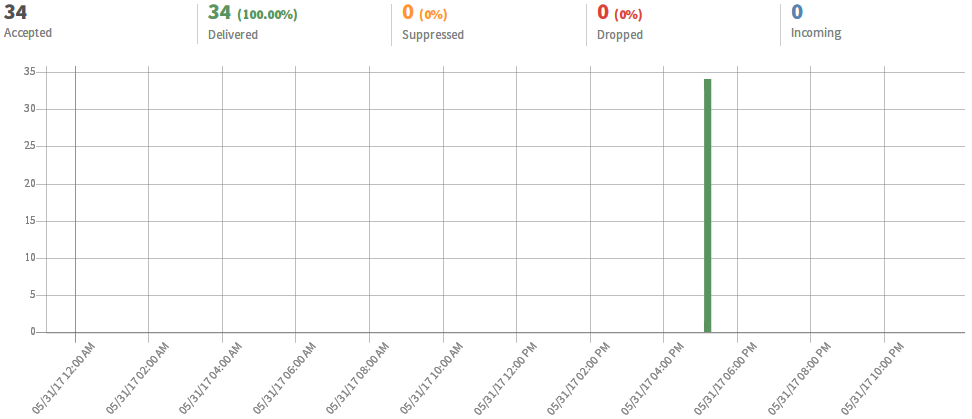
\includegraphics[width=0.9\textwidth]{mailgun_result.png}
    \caption{A screenshot showing the extent of the previous load-test (see fig. \ref{fig:pen-test}) in the Mailgun dashboard. Obviously, the build pipeline was triggered \emph{34} times, leading to the same number of E-Mails being sent. Out of this 34 E-Mails, \emph{8} showed a success message, whereas the others mostly failed due to other concurrent requests deleting the CWD as a preparation step prior to downloading the repository archive.}
    \label{fig:mailgun-result}
\end{figure}
%

\subsection{Load testing}
To evaluate the basic stability while handling multiple concurrent requests, the API was put under a high load test using Artillery\footnote{\url{https://artillery.io} -- Website of Artillery, a load testing toolkit.} (see fig. \ref{fig:pen-test}). Without any load balancing, nor any other high load supporting tool, 1200 POST requests triggered the build pipeline for a total duration of 60 seconds. As explained in the graphic's caption, the penetration test showed a success rate of roughly 1\%, a reasonable minimal response time of about 5 seconds but a terrible maximum response time of 51 seconds.

Of course, this data may not be interpreted as successful result in the first place, but it has to be stated, that the test was run on the endpoint causing the heaviest task in the system and most failure responses were effected by GitHub blocking most requests due to their rate abuse checking system.

The same test running on a much lighter task is showing a different picture; 1200 GET requests for receiving information about the latest build cycle had a response rate of 100\%. The response time ranged from 3 to 13 seconds, which is again a sign to not let a single application handle such an amount of requests without load balancing beforehand. In the end, it is safe to say, that the REST API may handle a reasonable amount of requests quite well on its own (e.g. requests triggered by GitHub webhooks), but consisting of multiple instances may be the best option for handling a significant amount of requests every once in a while.
